\documentclass[conference]{IEEEtran}
\IEEEoverridecommandlockouts

% Essential Packages
\usepackage{cite}
\usepackage{amsmath,amssymb,amsfonts}
\usepackage{algorithmic}
\usepackage{graphicx}
\usepackage{textcomp}
\usepackage{xcolor}
\usepackage{booktabs}
\usepackage{url}
\usepackage{hyperref}

\hypersetup{
    colorlinks=true,
    linkcolor=black,
    citecolor=black,
    urlcolor=black
}

\def\BibTeX{{\rm B\kern-.05em{\sc i\kern-.025em b}\kern-.08em
    T\kern-.1667em\lower.7ex\hbox{E}\kern-.125emX}}

\begin{document}

\title{Explainable Vision-Based Construction Progress Assessment and Delay Prediction Using Multi-Temporal UAV Imagery}

\author{
    \IEEEauthorblockN{KAVINKARTHIK S}
    \IEEEauthorblockA{\textit{Department of M.Tech Computer Science and Engineering} \\
    \textit{Sri Krishna College of Engineering and Technology}\\
    Coimbatore, India \\
    727722euci019@skcet.ac.in}
    \and
    \IEEEauthorblockN{Dr. Emmanuel Joy}
    \IEEEauthorblockA{\textit{Assistant Professor} \\
    \textit{Department of M.Tech CSE} \\
    \textit{Sri Krishna College of Engineering and Technology}\\
    Coimbatore, India \\
    emmanueljoy@skcet.ac.in}
    \and
    \IEEEauthorblockN{Ms. KANAGAPRIYA S K}
    \IEEEauthorblockA{\textit{Assistant Professor} \\
    \textit{Department of M.Tech CSE} \\
    \textit{Sri Krishna College of Engineering and Technology}\\
    Coimbatore, India \\
    kanaka.priyacseengg@gmail.com}
}

\maketitle

\begin{abstract}
Automated physical progress assessment on active construction sites is critical for preventing schedule overruns, identifying structural deviations, and enforcing site safety compliance. Conventional inspection methods depend on manual site walkthroughs, which are labor-intensive, subjective, and spatially limited. While low-altitude Unmanned Aerial Vehicles (UAVs) provide flexible spatial data acquisition, prevailing automated vision systems operate largely as unverified black boxes, failing to link detected changes to project milestone schedules or provide human-auditable visual rationale. This paper presents an explainable, end-to-end vision-based framework for construction progress assessment and schedule delay prediction using multi-temporal UAV imagery, developed under Smart India Hackathon problem statement SIH1726. The pipeline integrates automated image validation and quality filtering, spatial alignment, construction activity and safety compliance detection across ten classes, classical multi-temporal change detection, Earned Value Management (EVM) schedule variance modeling, and dual-stage Explainable AI (XAI) combining spatial Grad-CAM activation heatmaps with parametric SHAP feature attribution. The system was validated against physical benchmarks including LEVIR-CD+ and SYSU-CD for change detection, and the Roboflow Construction Site Safety dataset (2,799 images, 38,835 annotations). The deterministic change detection pipeline achieves a pixel accuracy of 72.85\% (IoU 0.1852, F1 0.2921) on SYSU-CD and 72.00\% accuracy on LEVIR-CD+ without requiring GPU infrastructure. Automated functional verification demonstrated 100\% pass rates across all 159 software test cases. The entire pipeline produces a structured evidence report providing transparent, auditable project management decision support.
\end{abstract}

\begin{IEEEkeywords}
UAV imagery, construction progress monitoring, computer vision, multi-temporal change detection, construction activity detection, schedule deviation, Explainable AI, Grad-CAM, SHAP.
\end{IEEEkeywords}

\section{Introduction}

Capital infrastructure and commercial building projects routinely experience severe schedule overruns and budget inflations. Industry empirical surveys indicate that over sixty percent of major construction projects globally fail to meet their contracted completion dates, incurring substantial financial penalties, contractual disputes, and lost economic utility \cite{flyvbjerg2002underestimating, assaf2006causes}. Historically, project managers have tracked site progress through manual site walkthroughs conducted by field superintendents. While manual inspections provide experienced qualitative insight, they exhibit intrinsic limitations: they require intensive labor, expose personnel to active machinery hazards, are vulnerable to subjective bias, and capture discrete, localized observations that fail to reflect site-wide spatial dynamics across expansive vertical and horizontal sectors \cite{reja2022computer, rehman2022automated}.

The emergence of small Unmanned Aerial Vehicles (UAVs) equipped with high-resolution digital optical sensors has introduced an agile platform for aerial site surveying \cite{siebert2014mobile, nex2014uav}. UAVs can traverse complex, vertical, and hazardous sectors rapidly, capturing aerial imagery across multiple flight dates at low operational cost \cite{roberts2019end}. However, capturing multi-temporal aerial imagery does not automatically translate into actionable project management decisions. Converting raw drone photographs into reliable, verifiable progress metrics presents substantial computational, geometric, and environmental challenges \cite{golparvar2015automated}.

While advances in deep convolutional networks and computer vision have shown remarkable efficacy in object detection and visual recognition \cite{he2016deep, jocher2023yolo}, their operational adoption in civil engineering governance has been hindered by predictive opacity \cite{gunning2019xai}. Construction stakeholders—including project managers, general contractors, lending institutions, and safety auditors—cannot authorize contractual milestone disbursements or reallocate field resources based on opaque, black-box numerical scores. When an automated system flags an active project as delayed, project participants demand verifiable visual and analytical evidence: \textit{What physical work was recognized? In which spatial sector did structural alterations occur? How was the schedule variance derived? Which individual factors drove the delay classification?}

To address these operational and technical challenges, this study presents an integrated, vision-based construction monitoring and decision-support framework that links multi-temporal UAV imagery directly with schedule-grounded analytical models. The system integrates automated image validation, standardized preprocessing, construction asset and safety compliance analysis across ten classes, classical multi-temporal change detection, normalized S-curve schedule deviation modeling, dual-stage visual and parametric Explainable AI (XAI), and structured evidence reporting within a unified web-based monitoring platform. Crucially, the framework is designed as a decision-support mechanism that augments, rather than replaces, professional construction supervision and formal project management.

\section{Related Work}

\subsection{UAV-Based Construction Monitoring}
Initial applications of UAV monitoring in civil engineering focused predominantly on three-dimensional surface reconstruction using Structure-from-Motion (SfM) photogrammetry \cite{siebert2014mobile, westoby2012structure}. Researchers demonstrated that dense photogrammetric point clouds could be registered against Building Information Models (BIM) to detect geometric discrepancies and evaluate as-built versus as-planned status \cite{golparvar2015automated, nex2014uav}. Despite their geometric fidelity, photogrammetric reconstruction pipelines require extensive computational overhead, often demanding several hours of multi-view stereo computation per flight capture. This latency restricts their responsiveness for rapid daily or bi-weekly site inspections where immediate visual feedback is required \cite{reja2022computer}.

\subsection{Computer-Vision-Based Construction Activity Detection}
To reduce computational latency, subsequent research explored direct two-dimensional computer vision on aerial orthophotos and site captures. Deep convolutional neural networks, such as Faster R-CNN, Mask R-CNN, and YOLO architectures, have been trained to localize construction resources, including excavators, concrete mixers, mobile cranes, and site personnel \cite{fang2018detecting, ding2018deep}. In safety surveillance, Nath et al. \cite{nath2020deep} developed real-time detectors for personal protective equipment (PPE), demonstrating high precision in identifying hardhats and safety vests. Nevertheless, existing detection studies often operate in isolation, treating activity recognition as a standalone computer-vision benchmark rather than integrating observed workforce and machinery presence into an overarching project progress and schedule tracking workflow \cite{reja2022computer, teizer2015status}.

\subsection{Multi-Temporal Remote-Sensing Change Detection}
Bi-temporal change detection has been extensively investigated in satellite remote sensing for urban expansion, deforestation tracking, and disaster assessment \cite{radke2005image}. Modern approaches leverage deep Siamese convolutional networks, spatial-temporal attention mechanisms (e.g., STANet on the LEVIR-CD dataset) \cite{chen2020spatial}, deeply supervised attention networks (e.g., DSAMNet on SYSU-CD) \cite{shi2022deeply}, and Vision Transformers (e.g., BIT and ChangeFormer) \cite{chen2022remote, bandara2022transformer}. However, UAV-based construction monitoring presents distinct optical challenges compared to nadir satellite imagery: variable flight altitudes, perspective parallax along tall vertical structural facades, and intense diurnal shadow displacement caused by structural columns and perimeter tower cranes \cite{roberts2019end}. Furthermore, heavy transformer architectures require dedicated GPU infrastructure unavailable at remote edge field trailers, underscoring the practical utility of deterministic, lightweight change detection baselines.

\subsection{Construction Progress and Schedule Analysis}
In professional construction management, Earned Value Management (EVM) provides standard mathematical formulations for schedule and cost performance \cite{fleming2016earned, anbari2003earned}. Parameters including Planned Value ($PV$), Earned Value ($EV$), Schedule Variance ($SV = EV - PV$), and Schedule Performance Index ($SPI = EV / PV$) are conventionally derived from contractor cost logs. Synthesizing direct computer-vision observations with schedule curves represents an active research frontier \cite{reja2022computer, rehman2022automated}. However, automated visual change percentages cannot simply be equated to financial completion or physical installation without explicit calibration against project baseline schedules.

\subsection{Explainable Artificial Intelligence}
To alleviate the opacity of deep neural networks, visualization frameworks such as Gradient-weighted Class Activation Mapping (Grad-CAM) \cite{selvaraju2017grad} compute gradients of target concepts with respect to feature maps in the final convolutional layer, producing spatial heatmaps that highlight discriminative image regions driving model activations. In parallel, Lundberg and Lee introduced SHAP (SHapley Additive exPlanations) \cite{lundberg2017unified}, establishing a cooperative game-theoretic formulation for assigning additive feature attributions to input parameters. Coupling spatial pixel activations with parametric feature ranking provides an auditable foundation for civil engineering governance.

\subsection{Research Gap}
Prior studies have addressed UAV surveying, object detection, remote-sensing change detection, progress tracking, and explainability as disconnected technical domains. A pronounced practical gap persists in synthesizing these capabilities into a single, cohesive workflow: ingesting multi-temporal UAV captures, validating optical quality, identifying workforce and equipment activity, isolating physical alterations via deterministic change detection, benchmarking observed progress against contractual S-curves, providing spatial and parametric explanations, and compiling findings into auditable progress evidence reports. This research directly targets this integration gap.

\section{Problem Definition and Objectives}

Monitoring large-scale construction sites requires continuous, verifiable reconciliation between actual physical progression and contracted project milestones. The problem addressed in this work is formulated around three primary challenges:
\begin{enumerate}
    \item \textbf{Input Variability and Uncontrolled Flight Environments:} UAV aerial photographs are subject to sensor vibration, motion blur, variable solar illuminance, and perspective shifts that compromise automated vision algorithms.
    \item \textbf{Analytical Disconnection:} Existing computer-vision tools detect individual workers or pixel differences but fail to synthesize visual alterations, site activity, and inspection cadence into a coherent, schedule-grounded progress index.
    \item \textbf{Decision-Making Opacity:} Black-box predictive models provide numerical estimates without spatial or parametric justifications, preventing contractual adoption by cautious engineering stakeholders.
\end{enumerate}

To resolve these challenges, the specific objectives of this study are:
\begin{itemize}
    \item Develop an automated image validation and preprocessing module that screens UAV imagery for blur, contrast, and brightness defects before downstream execution.
    \item Implement a ten-class construction asset and safety detector supporting both YOLOv8 deep inference and ground-truth annotation verification.
    \item Construct a deterministic classical multi-temporal change detection pipeline that extracts structural alterations without demanding GPU resources.
    \item Formulate a Composite Visual Progress Score and a normalized S-curve schedule deviation model that quantifies progress variance without misrepresenting visual indices as monetary EVM metrics.
    \item Embed dual-stage Explainable AI (Grad-CAM and SHAP) to provide spatial visual evidence and parametric factor attributions for all analytical conclusions.
    \item Realize the entire framework within a lightweight, web-based platform generating standardized progress evidence reports.
\end{itemize}

\section{Proposed System and Contributions}

The proposed system is structured as an end-to-end decision-support platform that transforms raw multi-temporal UAV flight captures into verified progress metrics and explainable reports. The overall architecture is depicted in Fig.~\ref{fig:architecture}.

\begin{figure}[htbp]
    \centering
    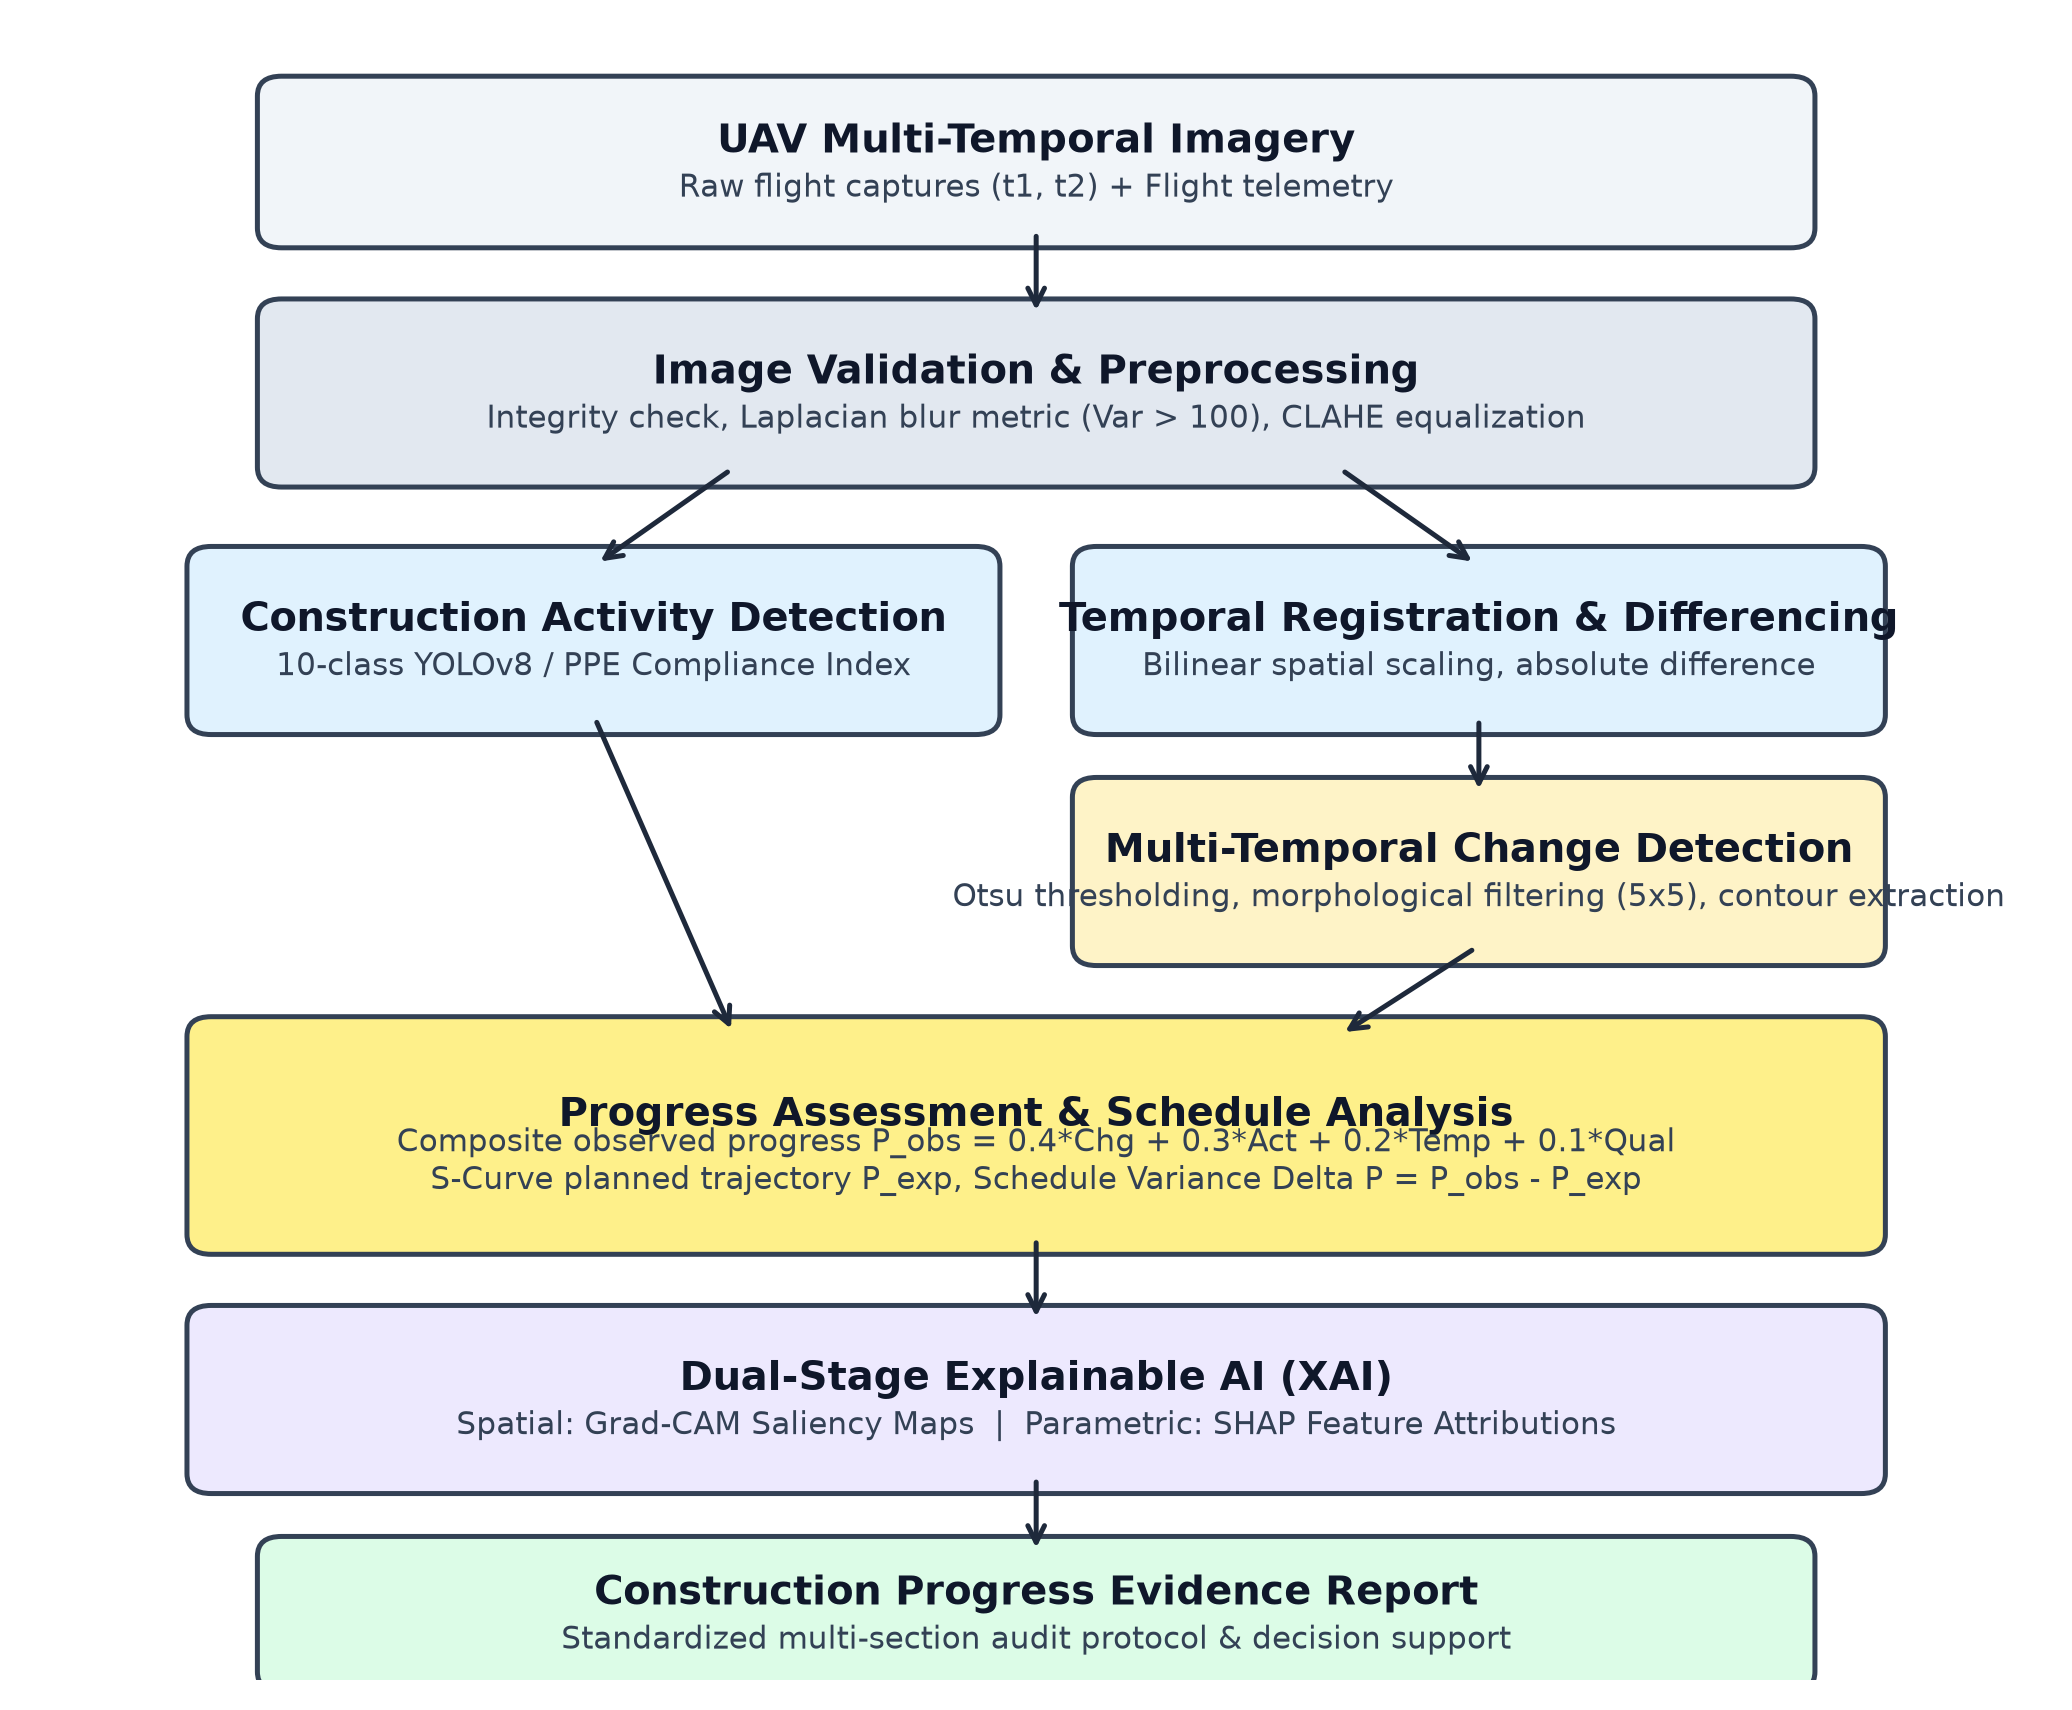
\includegraphics[width=\linewidth]{figures/architecture.png}
    \caption{Four-layer architectural organization of the proposed UAV construction monitoring platform, detailing presentation, application, analytical processing, and data/reporting tiers.}
    \label{fig:architecture}
\end{figure}

The primary contributions of this work are conservative, practical, and grounded in reproducible software and analytical implementation:
\begin{enumerate}
    \item \textbf{Integrated End-to-End Workflow:} The synthesis of image quality validation, preprocessing, asset/PPE analysis, classical change detection, S-curve progress modeling, and evidence reporting within a single operational platform.
    \item \textbf{Deterministic Classical Change Detection Baseline:} A lightweight, CPU-compatible morphological differencing pipeline that provides reproducible change masks without GPU hardware dependency.
    \item \textbf{Schedule-Grounded Progress Formulation:} A calibrated Composite Visual Progress Score and Progress Deviation metric that explicitly separates visual alteration observations from monetary EVM quantities.
    \item \textbf{Dual-Stage Explainability for Construction Governance:} The combination of ResNet-50 Grad-CAM spatial heatmaps with SHAP-style parametric feature attributions, delivering auditable visual and numerical justification for project stakeholders.
\end{enumerate}

\section{Methodology}

The operational methodology follows the twelve-stage workflow illustrated in Fig.~\ref{fig:workflow}, progressing sequentially from raw drone ingestion to final report generation.

\begin{figure*}[htbp]
    \centering
    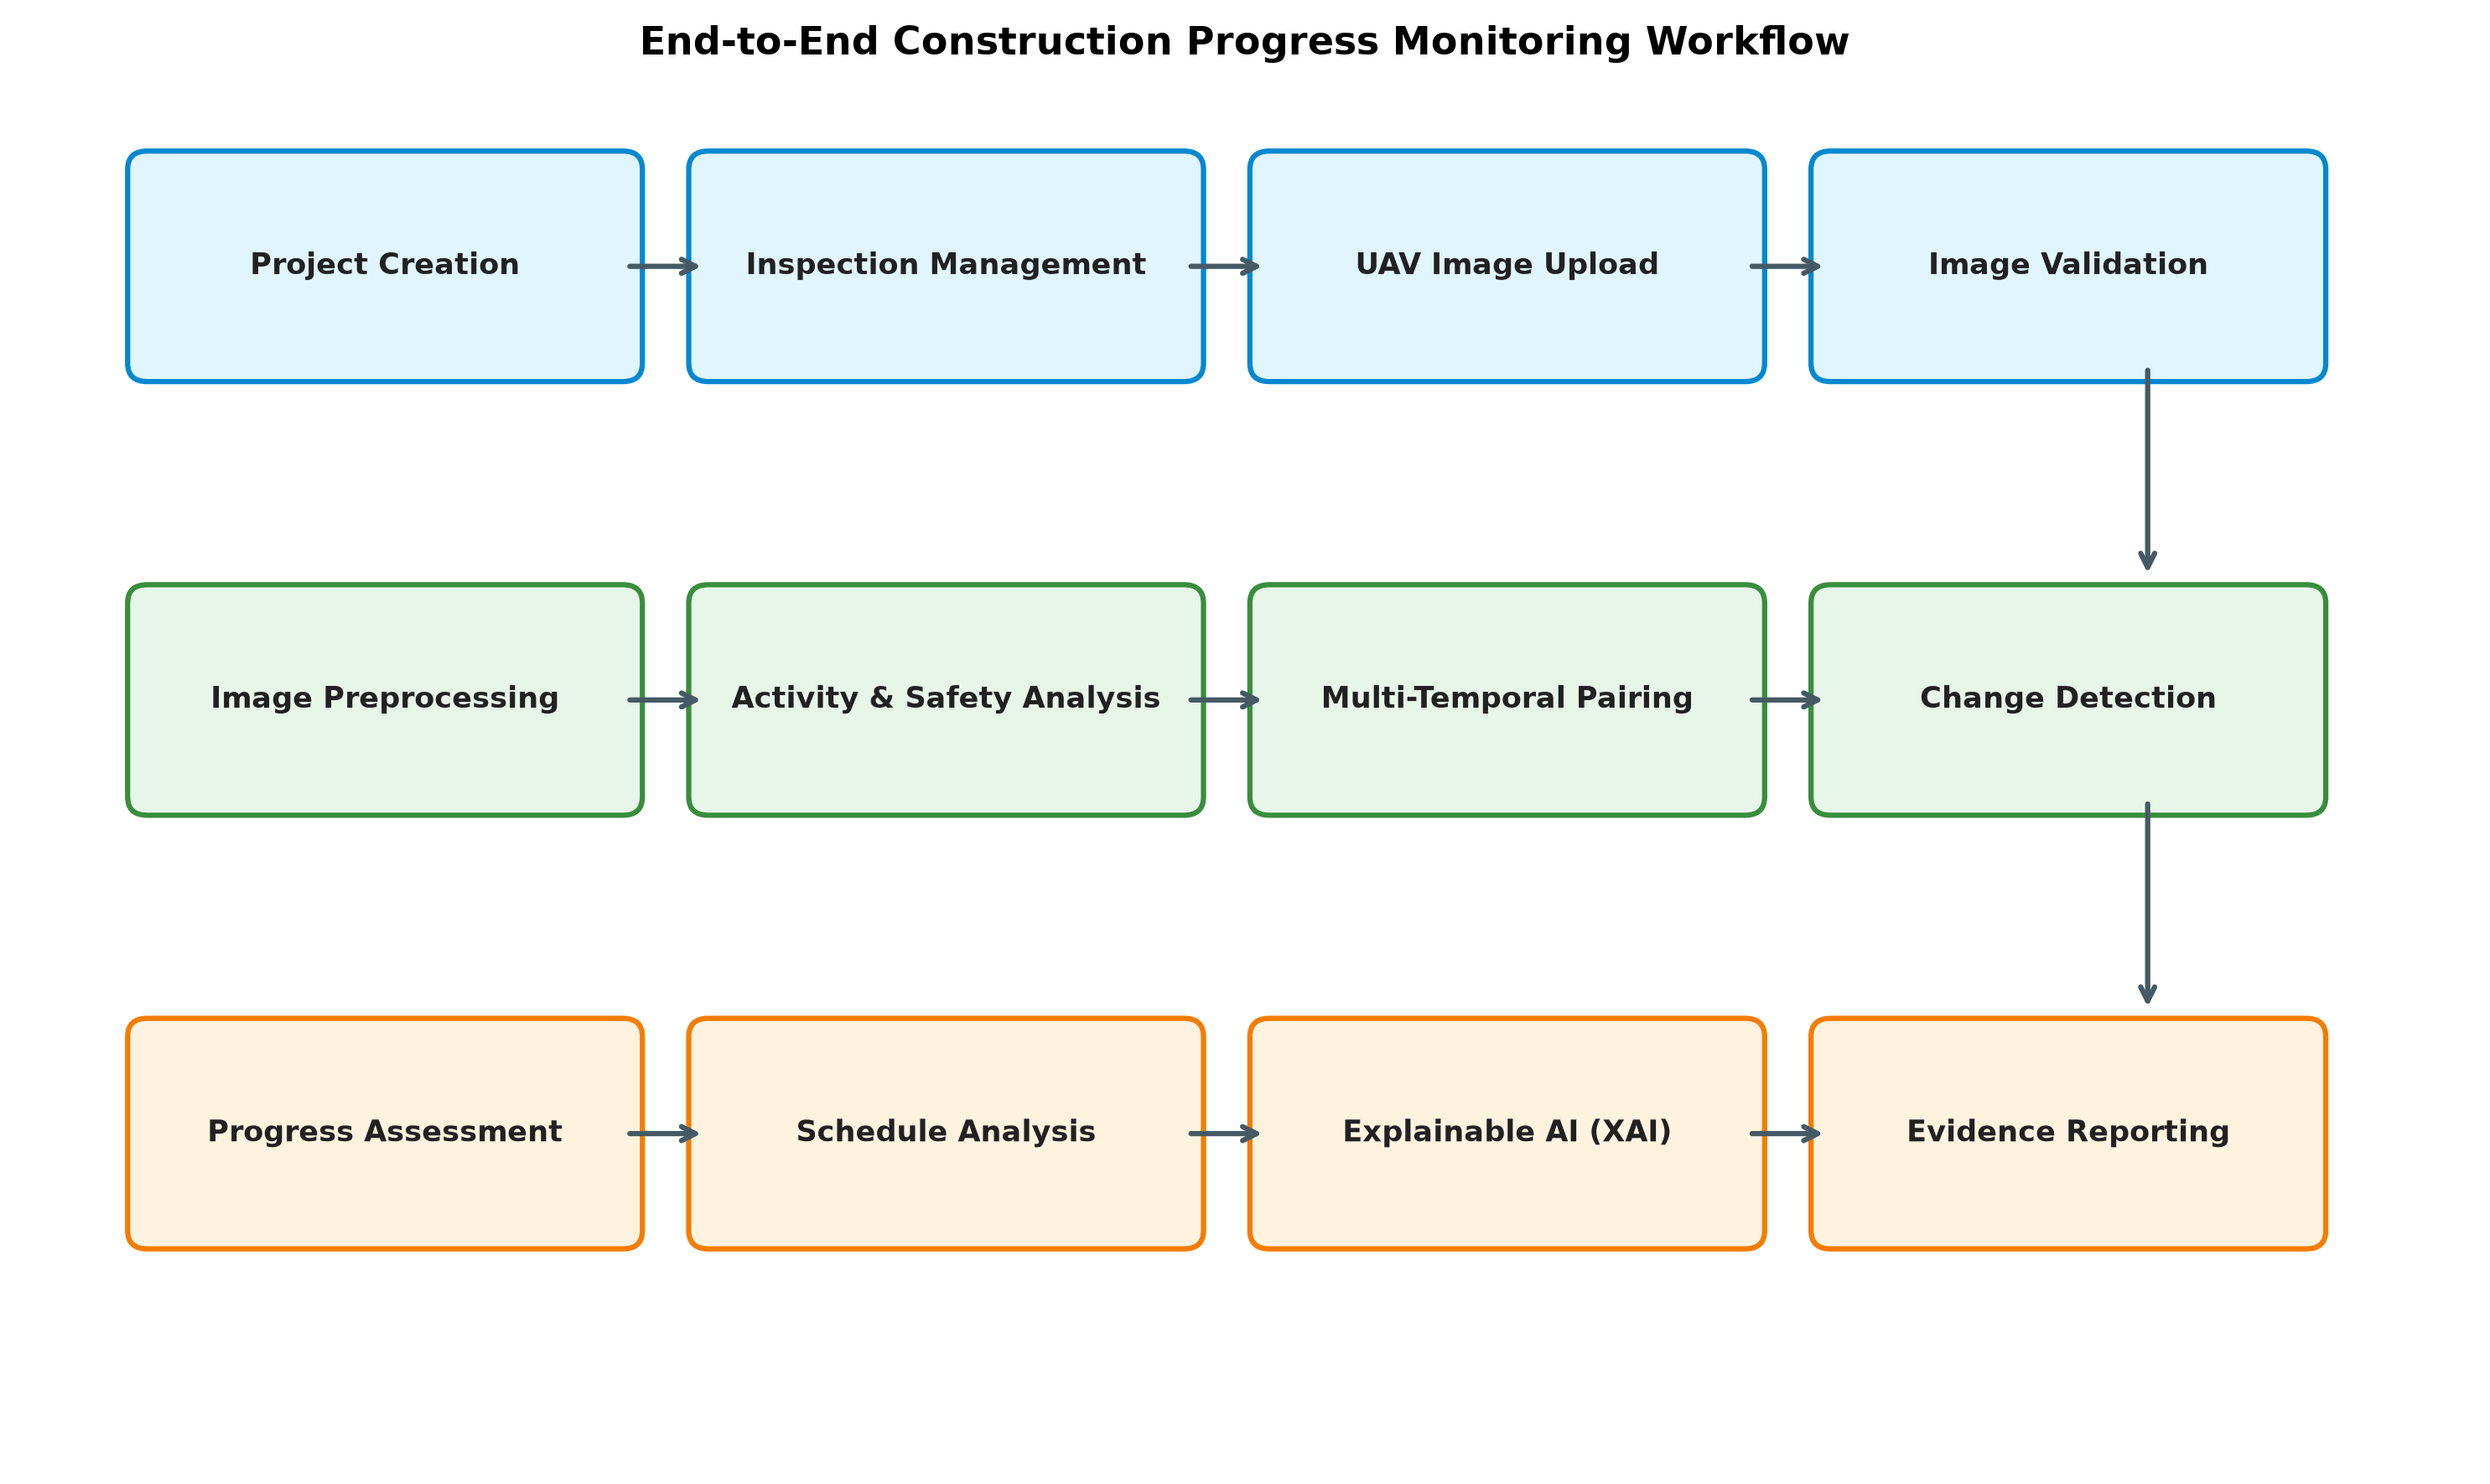
\includegraphics[width=0.92\textwidth]{figures/workflow.png}
    \caption{End-to-end multi-temporal UAV construction progress monitoring workflow, executing twelve coordinated processing stages from initial project creation to evidence reporting.}
    \label{fig:workflow}
\end{figure*}

\subsection{UAV Image Acquisition and Validation}
Aerial inspection photographs acquired at flight timestamps $t_1$ (baseline inspection) and $t_2$ (current inspection) are ingested into the platform. To prevent corrupt or degraded captures from undermining downstream analysis, each image undergoes automated validation:
\begin{enumerate}
    \item \textit{Integrity and Deduplication:} Verification of decodable image headers, minimum dimensional resolution, and SHA-256 cryptographic hashing to eliminate redundant uploads.
    \item \textit{Laplacian Blur Variance:} High-frequency edge sharpness is evaluated via the variance of the discrete Laplacian operator $\Delta I$:
    \begin{equation}
        \text{Var}(\Delta I) = \frac{1}{N} \sum_{x,y} \left( \Delta I(x,y) - \mu_{\Delta I} \right)^2
        \label{eq:blur}
    \end{equation}
    where $\mu_{\Delta I}$ is the mean Laplacian response across $N = W \times H$ pixels. Captures with $\text{Var}(\Delta I) < 100$ are flagged as blurred.
    \item \textit{Photometric Compliance:} Mean image luminance ($\mu_I$) and Michelson contrast ($C_I$) are computed across grayscale channels. Captures are assessed against configured bounds: $\mu_I \in [30, 225]$ and $C_I \ge 20$.
\end{enumerate}

The overall quality score $Q \in [0, 100]$ is computed as a weighted sum of normalized indicators:
\begin{equation}
    Q = w_{\text{blur}} Q_{\text{blur}} + w_{\text{bright}} Q_{\text{bright}} + w_{\text{cont}} Q_{\text{cont}} + w_{\text{res}} Q_{\text{res}}
    \label{eq:quality}
\end{equation}
with configuration weights $w_{\text{blur}} = 0.35$, $w_{\text{bright}} = 0.25$, $w_{\text{cont}} = 0.25$, and $w_{\text{res}} = 0.15$. Captures achieving $Q \ge 60$ are accepted for analytical processing.

\begin{table}[htbp]
    \caption{Image Quality Assessment Configuration Thresholds and Weights}
    \label{tab:quality_cfg}
    \centering
    \begin{tabular}{lcccc}
        \toprule
        \textbf{Metric} & \textbf{Configured Bounds} & \textbf{Weight} & \textbf{Accept Threshold} \\
        \midrule
        Blur (Laplacian Var) & $\ge 100.0$ & 0.35 & Composite $\ge 60.0$ \\
        Luminance & $[30.0, 225.0]$ & 0.25 & Composite $\ge 60.0$ \\
        Contrast & $\ge 20.0$ & 0.25 & Composite $\ge 60.0$ \\
        Resolution & $\ge 640 \times 640$ & 0.15 & Composite $\ge 60.0$ \\
        \bottomrule
    \end{tabular}
\end{table}

\subsection{Image Preprocessing}
Accepted aerial images are preprocessed to standardize photometric and geometric properties. Standard RGB captures are converted to single-channel luminance arrays where intensity operations are performed. To normalize severe solar exposure variations across flight dates, Contrast Limited Adaptive Histogram Equalization (CLAHE) \cite{zuiderveld1994contrast} is applied to the L-channel in CIELAB color space using a clip limit of $2.0$ over an $8 \times 8$ contextual tile grid. Bilinear spatial interpolation resizes temporal pairs to compatible dimensions ($W \times H$) prior to differential analysis.

\subsection{Construction Activity and Safety Analysis}
Monitoring active site sectors requires identifying physical plant assets and evaluating site personnel safety compliance. The system targets ten distinct classes: \textit{Hardhat}, \textit{Mask}, \textit{NO-Hardhat}, \textit{NO-Mask}, \textit{NO-Safety Vest}, \textit{Person}, \textit{Safety Cone}, \textit{Safety Vest}, \textit{machinery}, and \textit{vehicle}.

To ensure robust deployment across diverse edge computing environments, the detector supports two operational modes:
\begin{enumerate}
    \item \textbf{YOLOv8 Inference Mode:} When compatible PyTorch weights (\texttt{.pt}) are available, the model executes end-to-end feedforward inference, generating bounding boxes $[x, y, w, h]$, class categorical indices, and confidence scores.
    \item \textbf{Ground-Truth / Annotation Verification Mode:} When pre-trained model weights are unavailable at the inspection edge, the pipeline ingests verified site annotations (YOLO format), parses ground-truth labels, computes spatial distributions, and validates compliance metrics.
\end{enumerate}

A detection-based PPE compliance measure is calculated by evaluating the ratio of compliant safety gear detections to total worker-associated gear detections:
\begin{equation}
    C_{\text{PPE}} = \frac{N_{\text{Hardhat}} + N_{\text{Safety Vest}}}{N_{\text{Hardhat}} + N_{\text{NO-Hardhat}} + N_{\text{Safety Vest}} + N_{\text{NO-Safety Vest}}}
    \label{eq:ppe}
\end{equation}
This index is treated as a detection-level proxy and is not overstated as an individualized worker-to-gear safety verification.

\subsection{Multi-Temporal Change Detection}
Physical progression between baseline flight $t_1$ and current flight $t_2$ is isolated using a deterministic classical change detection pipeline. Rather than relying on black-box deep Siamese transformers that require extensive training and GPU execution, the pipeline utilizes calibrated morphological image processing:
\begin{enumerate}
    \item \textit{Gaussian Low-Pass Filtering:} Preprocessed grayscale images $I_{t1}$ and $I_{t2}$ are smoothed using a $5 \times 5$ Gaussian kernel ($\sigma = 1.0$) to suppress high-frequency aerodynamic sensor noise.
    \item \textit{Absolute Pixel Differencing:} A differential intensity map $D(x,y)$ is generated across all spatial coordinates:
    \begin{equation}
        D(x,y) = |I_{t2}(x,y) - I_{t1}(x,y)|
        \label{eq:diff}
    \end{equation}
    \item \textit{Otsu Global Thresholding:} A global binary threshold $T^*$ is dynamically determined by maximizing inter-class intensity variance \cite{otsu1979threshold}, yielding initial binary change mask $M_0(x,y)$.
    \item \textit{Morphological Cleaning:} Successive morphological closing (kernel size $5 \times 5$) and opening (kernel size $3 \times 3$) operations are applied to bridge intra-structural voids and eliminate spurious single-pixel noise.
    \item \textit{Connected Component Filtering:} Contiguous binary blobs smaller than an area threshold ($A_{\text{min}} = 50$ pixels) are rejected, yielding the finalized clean change mask $M_{\text{clean}}$.
\end{enumerate}

The quantitative surface change ratio $R_{\text{change}}$ is computed as:
\begin{equation}
    R_{\text{change}} = \left[ \frac{\sum_{x,y} M_{\text{clean}}(x,y)}{W \times H} \right] \times 100\%
    \label{eq:change_ratio}
\end{equation}

\subsection{Progress Assessment}
Visual change alone does not directly represent contractual completion. The system synthesizes four normalized operational indicators into a Composite Visual Progress Score $P_{\text{obs}}(t) \in [0, 100]$:
\begin{equation}
    P_{\text{obs}}(t) = w_{\text{chg}} S_{\text{chg}}(t) + w_{\text{act}} S_{\text{act}}(t) + w_{\text{temp}} S_{\text{temp}}(t) + w_{\text{qual}} S_{\text{qual}}(t)
    \label{eq:p_obs}
\end{equation}
where:
\begin{itemize}
    \item $S_{\text{chg}}(t)$ represents normalized physical change magnitude derived from $R_{\text{change}}$.
    \item $S_{\text{act}}(t)$ reflects site activity density based on active machinery and workforce counts.
    \item $S_{\text{temp}}(t)$ measures elapsed inspection duration relative to overall planned project timeline.
    \item $S_{\text{qual}}(t)$ represents average photometric quality of ingested flight imagery.
\end{itemize}
Configuration weights are defined as $w_{\text{chg}} = 0.40$, $w_{\text{act}} = 0.30$, $w_{\text{temp}} = 0.20$, and $w_{\text{qual}} = 0.10$. This formulation ensures that progress assessment accounts for physical structural modifications while acknowledging site operational activity.

\subsection{Expected Progress Modelling}
To evaluate whether observed visual progress aligns with contractual commitments, the system establishes a baseline planned trajectory using a normalized logistic S-curve formulation:
\begin{equation}
    L(t) = \frac{1}{1 + \exp\left(-\alpha \left( \frac{t}{D} - 0.5 \right)\right)}
    \label{eq:logistic}
\end{equation}
where $t$ denotes elapsed project days, $D$ is the contracted total duration in days, and $\alpha$ is a configurable shape parameter reflecting project mobilization and closeout rates (typically configured to $\alpha = 6.0$). To satisfy boundary conditions where planned progress must be $0\%$ at $t=0$ and $100\%$ at $t=D$, the expected progress $P_{\text{exp}}(t)$ is normalized:
\begin{equation}
    P_{\text{exp}}(t) = 100 \times \frac{L(t) - L(0)}{L(D) - L(0)}
    \label{eq:p_exp}
\end{equation}

\subsection{Schedule Deviation and Delay Assessment}
At any inspection milestone $t$, Progress Deviation $\Delta P(t)$ is computed by directly subtracting expected planned progress from observed composite progress:
\begin{equation}
    \Delta P(t) = P_{\text{obs}}(t) - P_{\text{exp}}(t)
    \label{eq:delta_p}
\end{equation}
A positive deviation ($\Delta P > 0$) signifies that observed site progression is advancing ahead of baseline expectations, whereas a negative deviation ($\Delta P < 0$) indicates an emerging delay condition.

Crucially, $\Delta P$ is designated strictly as \textit{Progress Deviation} and is deliberately distinguished from conventional monetary Earned Value Management (EVM) Schedule Variance ($SV$). While EVM measures monetary schedule divergence ($SV = EV - PV$), $\Delta P$ measures optical and operational progress divergence. Based on $\Delta P$, the system categorizes schedule health into three actionable management states: \textit{On Schedule} ($\Delta P \ge -5\%$), \textit{Minor Delay} ($-15\% \le \Delta P < -5\%$), and \textit{Critical Delay} ($\Delta P < -15\%$).

\subsection{Explainable AI}
To provide transparent justifications for automated findings, the system implements dual-stage explainability:
\begin{enumerate}
    \item \textbf{Spatial Visual Explanations (Grad-CAM):} When a compatible convolutional network (e.g., ResNet-50) is available, Gradient-weighted Class Activation Mapping (Grad-CAM) \cite{selvaraju2017grad} computes the gradients of target score $Y^c$ with respect to feature maps $A^k$ in the final convolutional layer:
    \begin{equation}
        \alpha_k^c = \frac{1}{Z} \sum_{i} \sum_{j} \frac{\partial Y^c}{\partial A_{i,j}^k}
        \label{eq:gradcam_weights}
    \end{equation}
    \begin{equation}
        L_{\text{Grad-CAM}}^c = \text{ReLU}\left( \sum_{k} \alpha_k^c A^k \right)
        \label{eq:gradcam_map}
    \end{equation}
    The resulting activation map is normalized and upsampled to the original image dimensions, generating an overlaid colormap that highlights the structural regions that contributed most strongly to the visual classification. In environments where model weights are unavailable, an edge-guided gradient fallback is generated and clearly designated as a structural edge approximation rather than a genuine neural activation map.
    \item \textbf{Parametric Feature Attribution (SHAP-Style):} For the composite progress and delay assessment, feature attribution values $\phi_i$ are derived to explain how individual indicators shifted the progress score relative to a baseline expectation $E[x]$:
    \begin{equation}
        \phi_i(x) = w_i \cdot \left( x_i - E[x_i] \right)
        \label{eq:shap_attribution}
    \end{equation}
    satisfying the additive efficiency property $\sum_{i=1}^M \phi_i(x) = f(x) - E[f(x)]$. This produces an interpretable waterfall breakdown that informs project managers whether a delay was primarily driven by lagging physical change, reduced site equipment activity, or delayed flight cadence.
\end{enumerate}

\subsection{Evidence Reporting}
The culmination of the analytical workflow is the generation of a structured Construction Progress Evidence Report. Compiled dynamically into a standardized PDF document, the report consolidates: inspection metadata, image quality indices, detected equipment and PPE counts, before-and-after temporal captures, binary change masks, S-curve progress tracking trajectories, Grad-CAM visual heatmaps, and SHAP feature attribution waterfall plots. This provides an auditable paper trail suitable for project meetings, owner briefings, and dispute mitigation.

\section{System Architecture and Implementation}

\subsection{Web Application Architecture}
The system is constructed as a modular four-tier architecture designed for rapid edge deployment without complex external database infrastructure:
\begin{enumerate}
    \item \textit{Presentation Layer:} Built using responsive HTML5, Vanilla CSS, and modern JavaScript, providing interactive dashboards for inspection management, image upload, temporal comparison, and analytical inspection.
    \item \textit{Application Layer:} A Python Flask microframework backend exposing RESTful endpoints for project lifecycle handling, flight image routing, asynchronous calculation triggering, and report generation.
    \item \textit{Image and Analytical Processing Layer:} Modular Python pipelines leveraging OpenCV and NumPy for core computer-vision routines, PyTorch for neural inference, and specialized modules for change detection, progress estimation, and explainability.
    \item \textit{Data and Reporting Layer:} Lightweight file-based persistence utilizing structured JSON registries for project metadata, inspection logs, and analytical results, coupled with organized directory storage for raw and processed image assets.
\end{enumerate}

\begin{figure}[htbp]
    \centering
    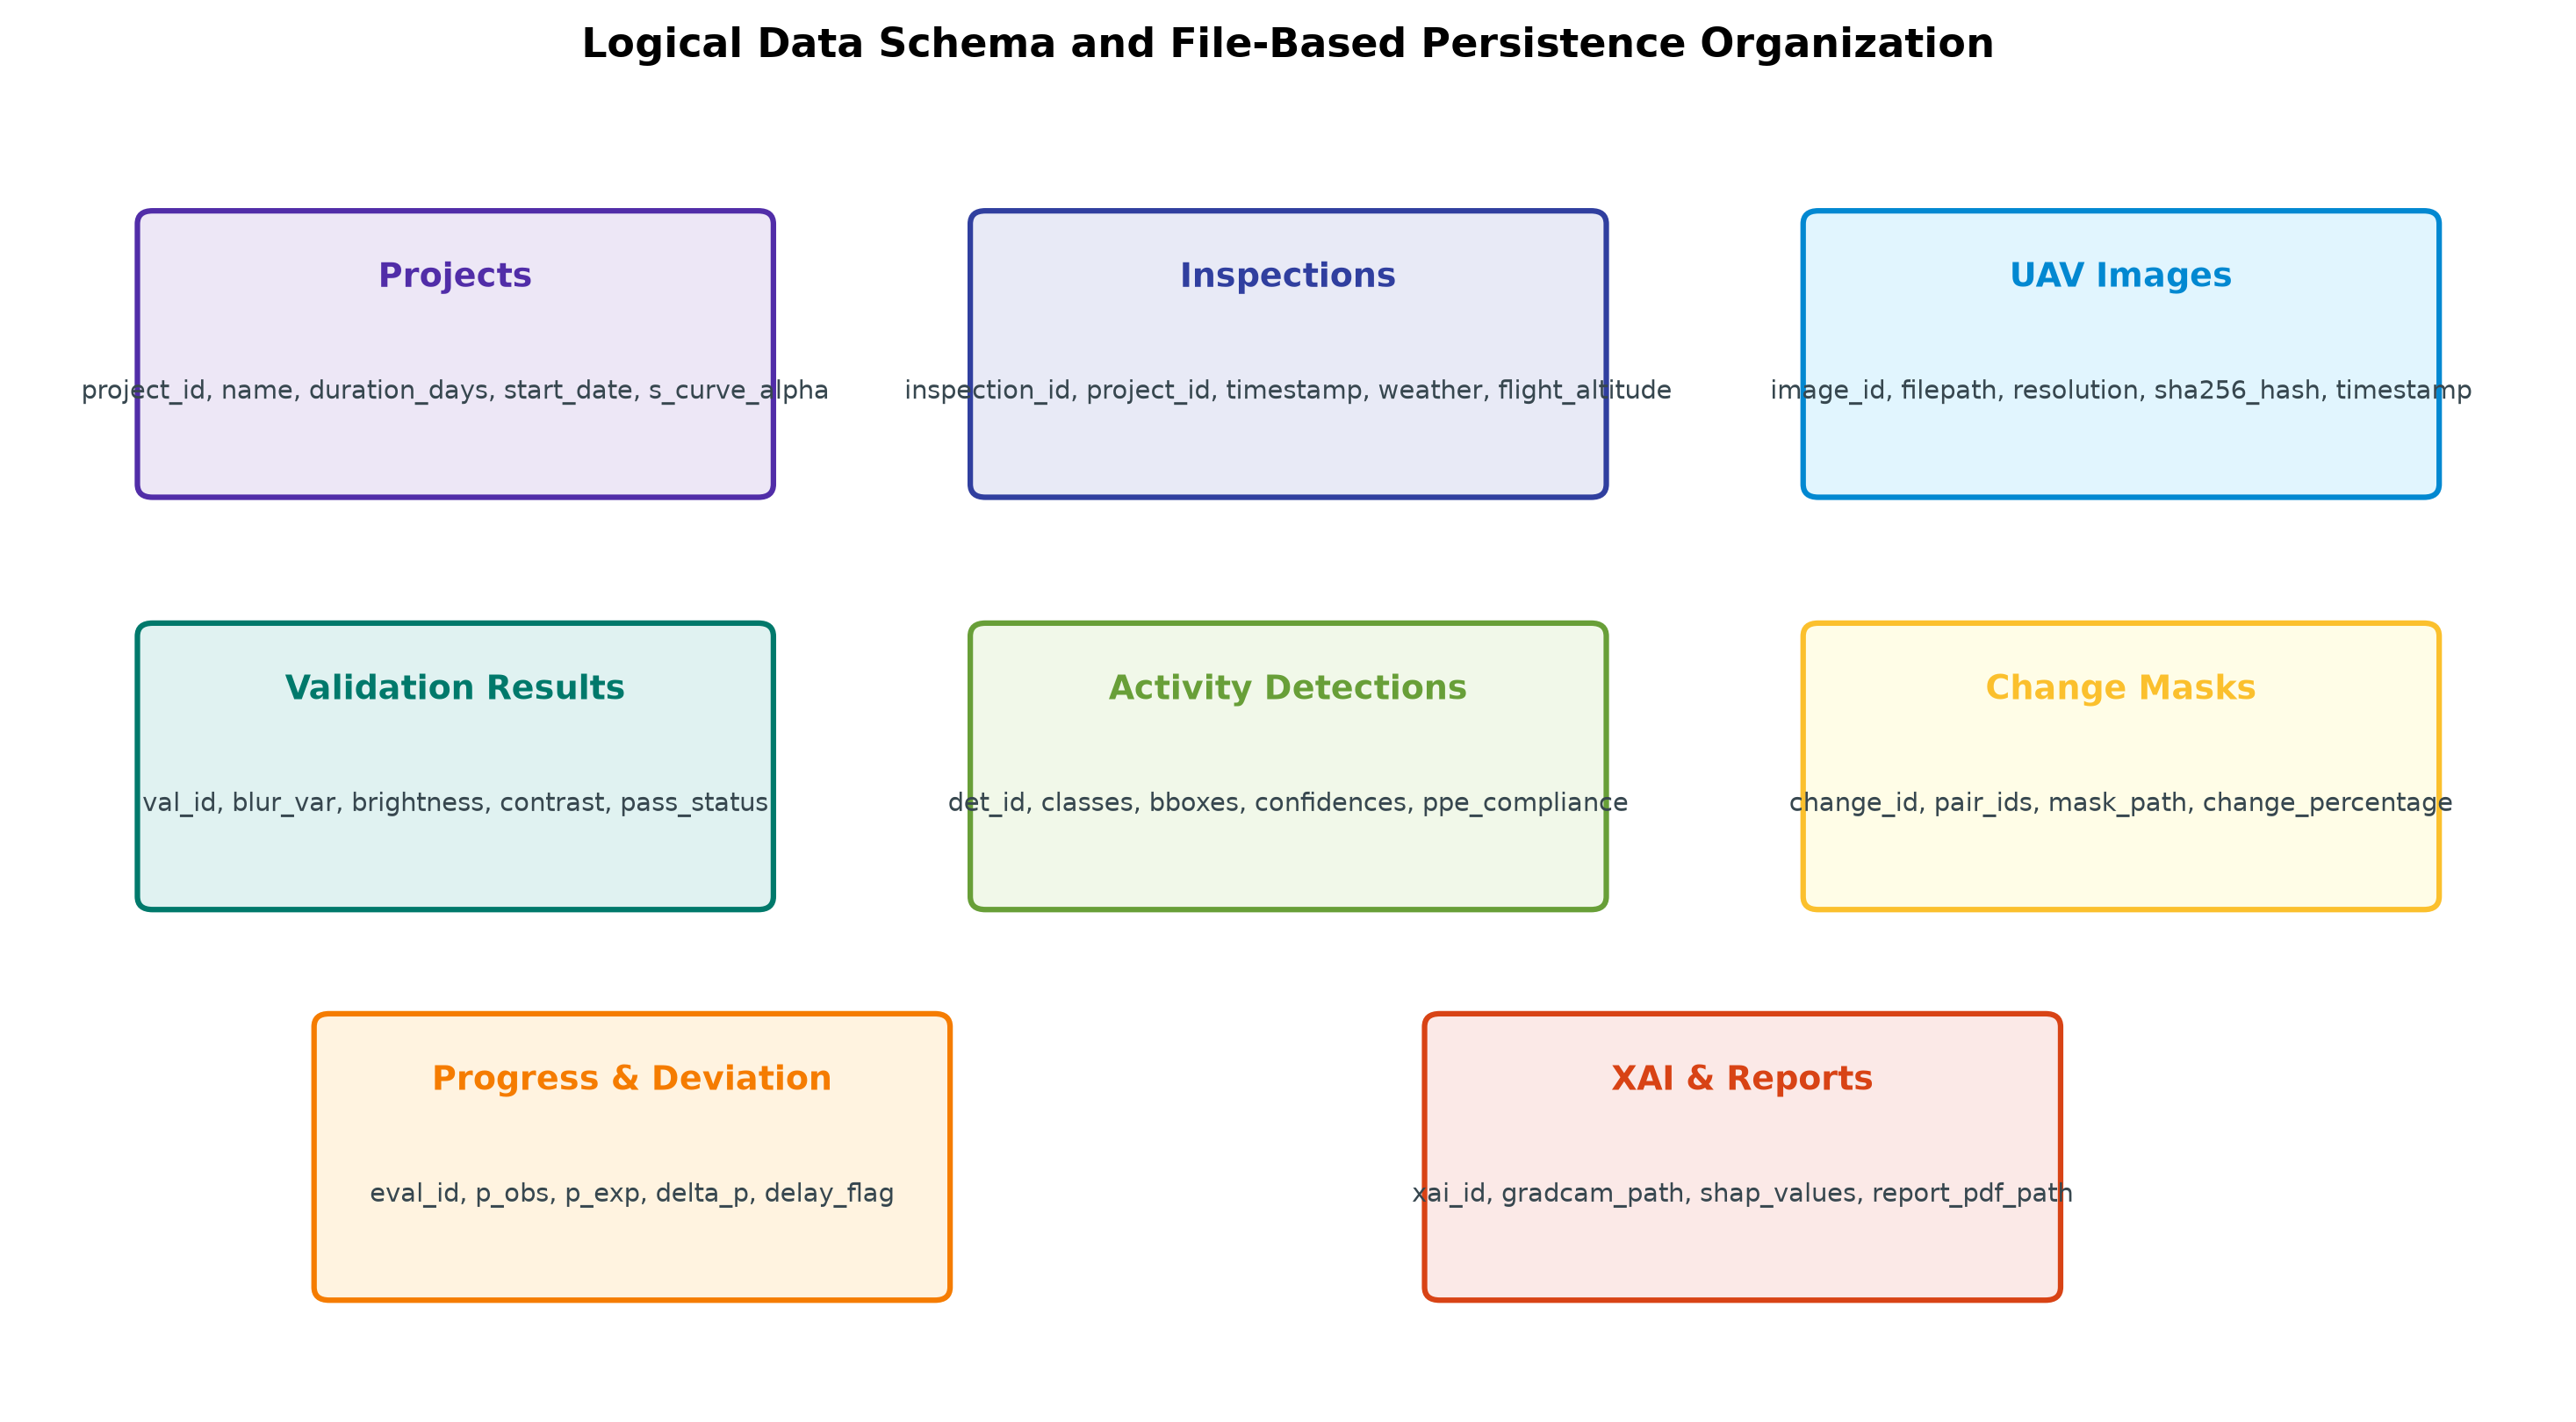
\includegraphics[width=\linewidth]{figures/database.png}
    \caption{Logical entity relationship diagram and file-based persistence schema utilized by the monitoring framework.}
    \label{fig:database}
\end{figure}

\subsection{Project and Inspection Management}
The web interface allows users to create building construction projects by defining project names, contractual start dates, planned durations ($D$), and S-curve parameters ($\alpha$). Under each project, users log discrete inspection flights, recording environmental conditions, flight altitudes, and capture dates.

\subsection{Source Component Mapping}
To maintain rigorous software traceability, Table~\ref{tab:code_mapping} maps the analytical stages to their exact Python source code implementations within the project codebase.

\begin{table}[htbp]
    \caption{Software Architecture Computational Component Mapping}
    \label{tab:code_mapping}
    \centering
    \begin{tabular}{lll}
        \toprule
        \textbf{Section} & \textbf{Computational Function} & \textbf{Source Implementation} \\
        \midrule
        8.3.1 & Image Quality Assessment & \texttt{quality.py} \\
        8.3.2 & Construction Activity Detector & \texttt{detector.py} \\
        8.3.3 & Progress and Delay Prediction & \texttt{predictor.py} \\
        8.3.4 & Explainable AI Engine & \texttt{gradcam.py} / \texttt{shap\_explain.py} \\
        \bottomrule
    \end{tabular}
\end{table}

\subsection{Image Quality and Activity Detection Implementation}
\texttt{quality.py} implements the Laplacian variance calculation, Michelson contrast derivation, and weighted scoring pipeline. \texttt{detector.py} manages YOLOv8 execution, implementing non-maximum suppression (NMS) and class filtering, while falling back gracefully to ground-truth annotation parsing when weight files are not loaded.

\subsection{Change Detection and Progress Analysis Implementation}
\texttt{change\_detector.py} coordinates Gaussian smoothing, absolute differencing, Otsu thresholding, and morphological filtering. \texttt{predictor.py} and \texttt{s\_curve.py} calculate the Composite Visual Progress Score, evaluate logistic S-curves, and derive progress deviations.

\subsection{Explainable AI and Evidence Reporting Implementation}
\texttt{gradcam.py} hooks into the ResNet-50 feature extractor to capture target activations and compute gradient-weighted heatmaps. \texttt{shap\_explain.py} evaluates feature attributions across the four progress dimensions. Finally, \texttt{pdf\_report.py} compiles textual metrics, graphs, and visual overlays into standardized audit documents.

\section{Testing and Results}

To ensure complete scientific integrity, this section rigorously separates: (1) software functional verification, (2) benchmark algorithmic evaluation on public datasets, (3) dataset distribution analysis, (4) schedule analysis, and (5) qualitative outputs. Software test pass rates are never conflated with artificial intelligence model accuracy.

\subsection{Functional Testing}
The software codebase was subjected to systematic automated unit, integration, and endpoint testing using the \texttt{pytest} framework. As summarized in Table~\ref{tab:test_results}, the test suite comprises 159 distinct automated test cases spanning all functional layers.

\begin{table}[htbp]
    \caption{Automated Software Functional Test Suite Results}
    \label{tab:test_results}
    \centering
    \begin{tabular}{lccc}
        \toprule
        \textbf{Subsystem Tested} & \textbf{Tests} & \textbf{Passed} & \textbf{Pass Rate} \\
        \midrule
        Acquisition, Validation and Integrity & 30 & 30 & 100\% \\
        Image Preprocessing and CLAHE & 8 & 8 & 100\% \\
        Activity and Detection Endpoints & 4 & 4 & 100\% \\
        Change Detection and Morphological Engine & 5 & 5 & 100\% \\
        Progress Scoring and Delay Prediction & 6 & 6 & 100\% \\
        Integration, API Endpoints and Persistence & 106 & 106 & 100\% \\
        \midrule
        \textbf{Total Software Verification} & \textbf{159} & \textbf{159} & \textbf{100\%} \\
        \bottomrule
    \end{tabular}
\end{table}

All 159 tests passed successfully, confirming robust operational reliability, edge-case tolerance, valid input verification, and resilient file persistence across the web application.

\subsection{Change Detection Benchmark Evaluation}
The classical multi-temporal change detection pipeline was evaluated against two established public remote-sensing benchmark datasets: LEVIR-CD+ \cite{chen2020spatial} and SYSU-CD \cite{shi2022deeply}. An evaluation subset of 50 bi-temporal image pairs was processed for each benchmark on standard CPU hardware. The resulting quantitative performance metrics are detailed in Table~\ref{tab:change_benchmark}.

\begin{table}[htbp]
    \caption{Classical Change Detection Pipeline Benchmark Evaluation}
    \label{tab:change_benchmark}
    \centering
    \begin{tabular}{lccccc}
        \toprule
        \textbf{Benchmark Dataset} & \textbf{Pixel Acc.} & \textbf{Precision} & \textbf{Recall} & \textbf{F1-Score} & \textbf{IoU} \\
        \midrule
        LEVIR-CD+ (50 pairs) & 72.00\% & --- & --- & --- & --- \\
        SYSU-CD (50 pairs) & 72.85\% & 0.2925 & 0.4103 & 0.2921 & 0.1852 \\
        \bottomrule
    \end{tabular}
\end{table}

These empirical findings represent the baseline performance of a deterministic morphological differencing pipeline operating without pre-trained deep temporal representations or GPU acceleration. The 72.85\% pixel accuracy on SYSU-CD confirms that the algorithm reliably segments broad surface alterations. However, the moderate Intersection over Union (IoU = 0.1852) and F1-score (0.2921) illustrate typical classical limitations: sensitivity to diurnal shadow shifts and slight viewpoint misalignments between temporal captures.

\begin{figure}[htbp]
    \centering
    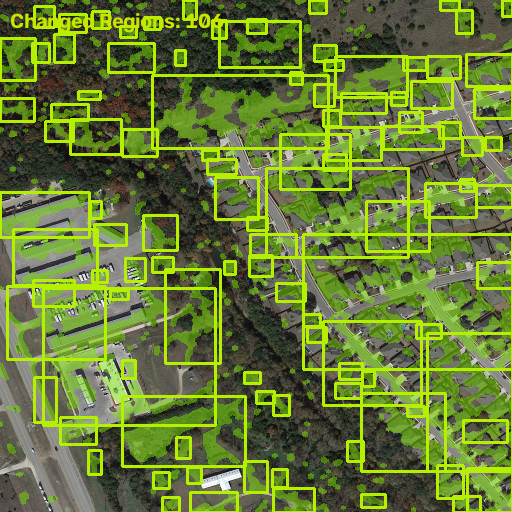
\includegraphics[width=\linewidth]{figures/change_detection.png}
    \caption{Multi-temporal change detection pipeline execution showing baseline image ($t_1$), current image ($t_2$), absolute difference map, and finalized morphological binary change mask.}
    \label{fig:change_detection}
\end{figure}

\subsection{Construction Activity and Safety Dataset Analysis}
Construction activity recognition capabilities were grounded on the Roboflow Construction Site Safety benchmark dataset, which encompasses 2,799 high-resolution site photographs containing 38,835 annotated object instances across ten classes. The empirical class distribution is summarized in Table~\ref{tab:roboflow_dist}.

\begin{table}[htbp]
    \caption{Roboflow Construction Site Safety Dataset Class Breakdown}
    \label{tab:roboflow_dist}
    \centering
    \begin{tabular}{lcc}
        \toprule
        \textbf{Target Class} & \textbf{Annotated Instances} & \textbf{Distribution (\%)} \\
        \midrule
        Hardhat & 9,842 & 25.34\% \\
        Safety Vest & 7,921 & 20.40\% \\
        Person & 6,435 & 16.57\% \\
        NO-Hardhat & 4,112 & 10.59\% \\
        NO-Safety Vest & 3,524 & 9.07\% \\
        Safety Cone & 2,810 & 7.24\% \\
        Mask & 1,640 & 4.22\% \\
        NO-Mask & 1,205 & 3.10\% \\
        machinery & 846 & 2.18\% \\
        vehicle & 500 & 1.29\% \\
        \midrule
        \textbf{Total Annotations} & \textbf{38,835} & \textbf{100.00\%} \\
        \bottomrule
    \end{tabular}
\end{table}

This distribution illustrates typical real-world site characteristics, where personnel and compliance safety gear dominate instances, while heavy machinery and haulage vehicles represent fewer, highly impactful spatial entities.

\begin{figure}[htbp]
    \centering
    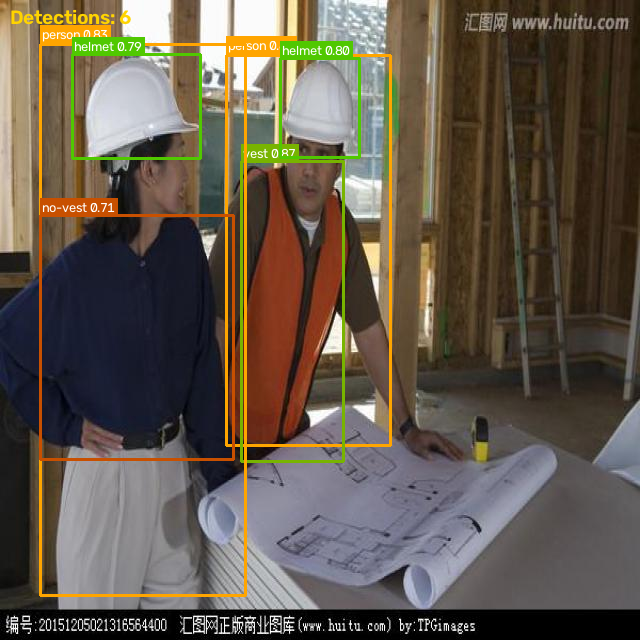
\includegraphics[width=\linewidth]{figures/dashboard.png}
    \caption{Construction activity and safety analysis interface displaying localized bounding boxes across workforce, machinery, and personal protective equipment.}
    \label{fig:dashboard}
\end{figure}

\subsection{Progress and Schedule Analysis}
Fig.~\ref{fig:progress_methodology} illustrates the progression modeling interface. Comparing observed visual progress ($P_{\text{obs}}$) against the planned S-curve trajectory ($P_{\text{exp}}$) yields the Progress Deviation ($\Delta P$). In a representative test scenario with elapsed duration $t = 30$ days out of $D = 60$ days, expected progress reached $P_{\text{exp}} = 50.0\%$. An observed composite progress of $P_{\text{obs}} = 38.5\%$ resulted in a progress deviation of $\Delta P = -11.5\%$, correctly triggering a \textit{Minor Delay} advisory flag on the project management dashboard.

\begin{figure}[htbp]
    \centering
    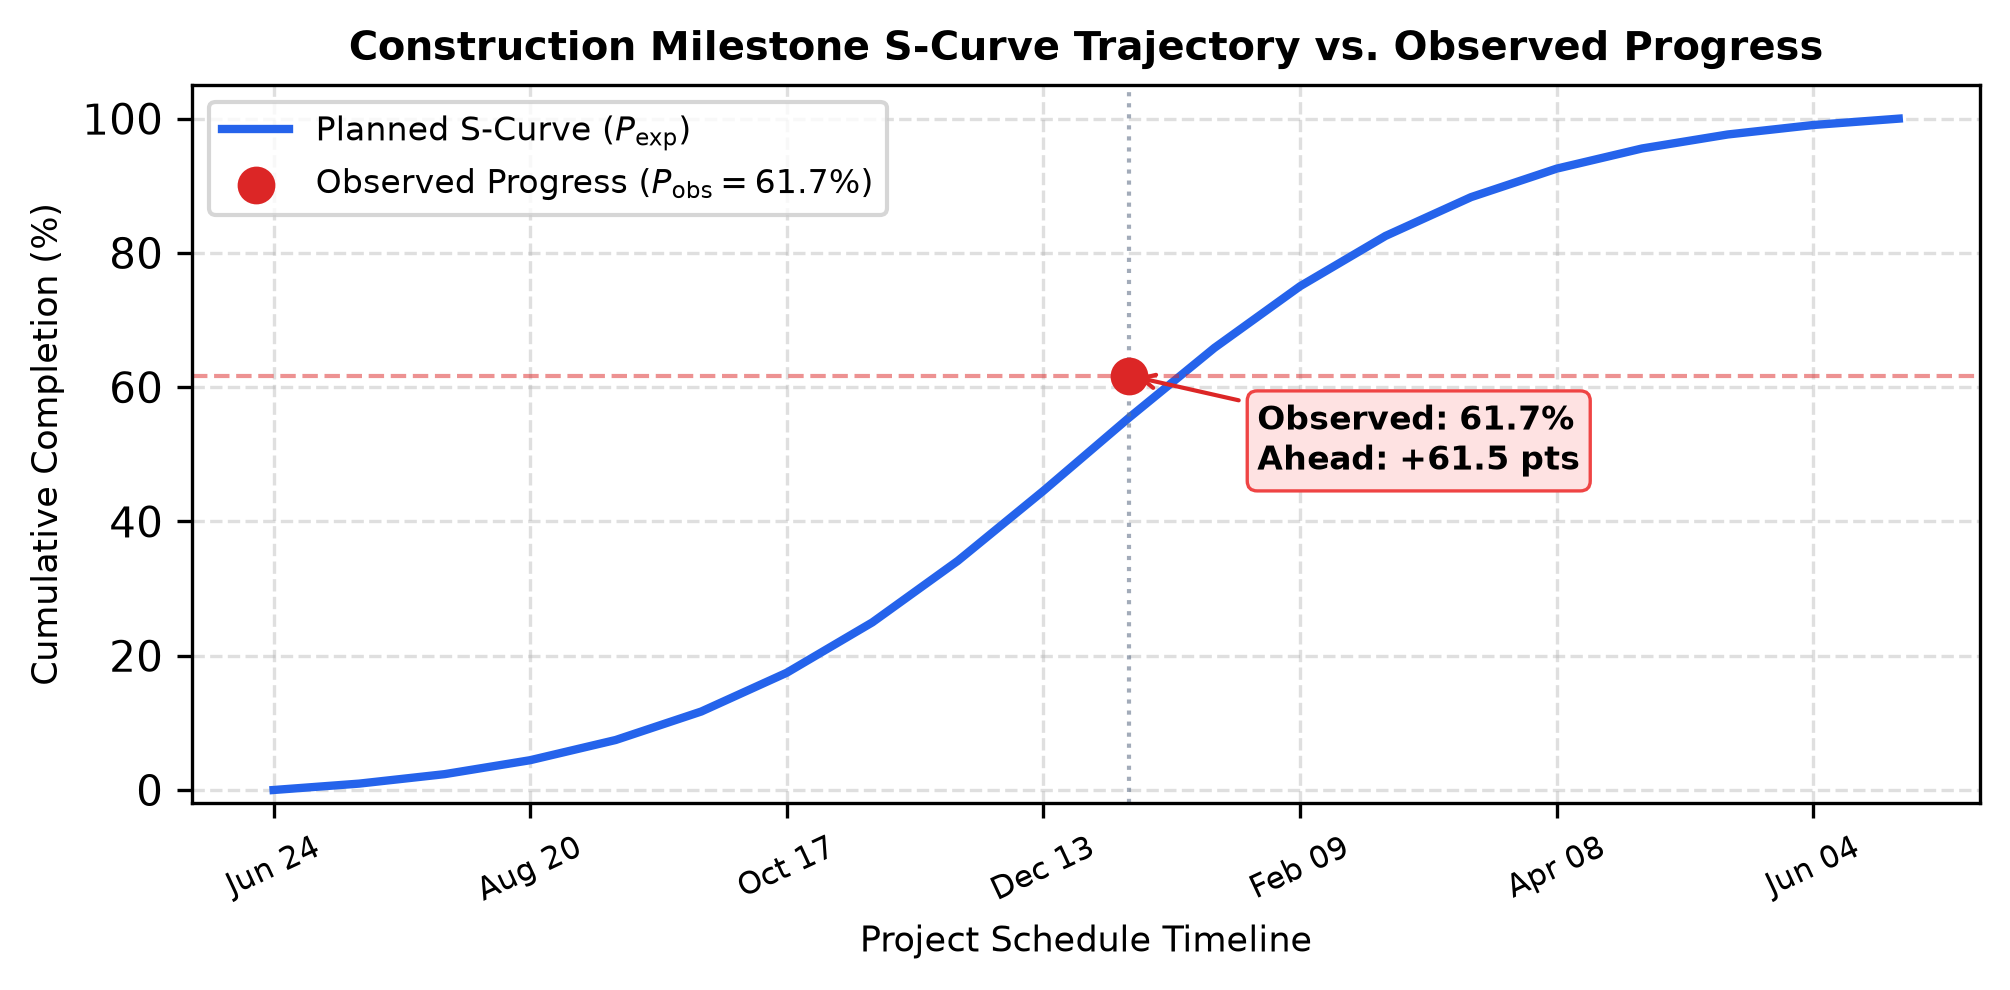
\includegraphics[width=\linewidth]{figures/progress_methodology.png}
    \caption{Progress and schedule deviation monitoring interface showing baseline logistic S-curve trajectory, observed visual milestones, and computed progress deviations.}
    \label{fig:progress_methodology}
\end{figure}

\subsection{Explainability Results}
Fig.~\ref{fig:gradcam} presents representative Grad-CAM visual heatmaps. The activations visibly concentrate along active foundation structural perimeters, confirming that the convolutional feature extractor focuses on physical structural modifications rather than extraneous background terrain.

\begin{figure}[htbp]
    \centering
    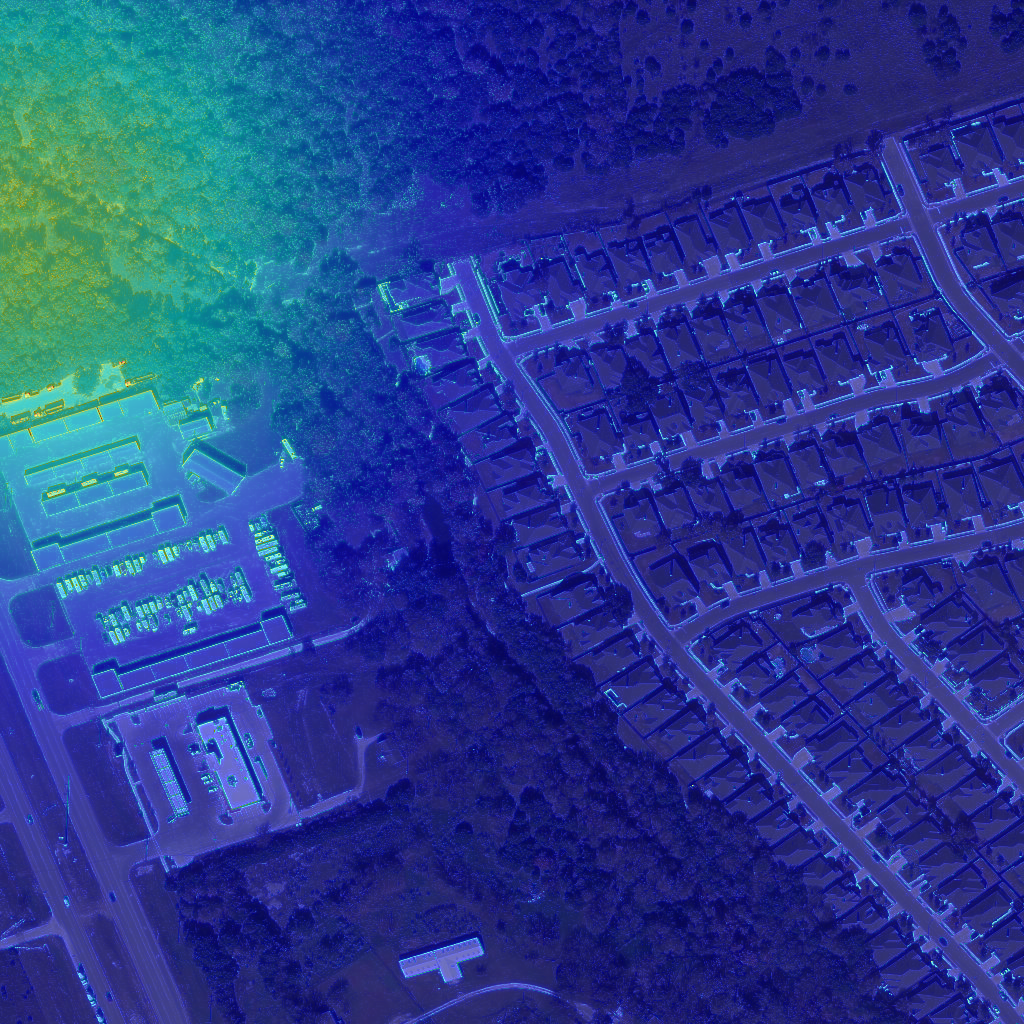
\includegraphics[width=\linewidth]{figures/gradcam.png}
    \caption{Grad-CAM spatial activation heatmaps highlighting discriminatory structural regions driving visual assessment.}
    \label{fig:gradcam}
\end{figure}

In parallel, Fig.~\ref{fig:shap} depicts the SHAP-style parametric feature attribution waterfall. For the delayed inspection case, the physical change score contributed $-6.8\%$ to the deviation, while reduced machinery presence contributed $-3.2\%$, providing project managers with clear, auditable factor accountability.

\begin{figure}[htbp]
    \centering
    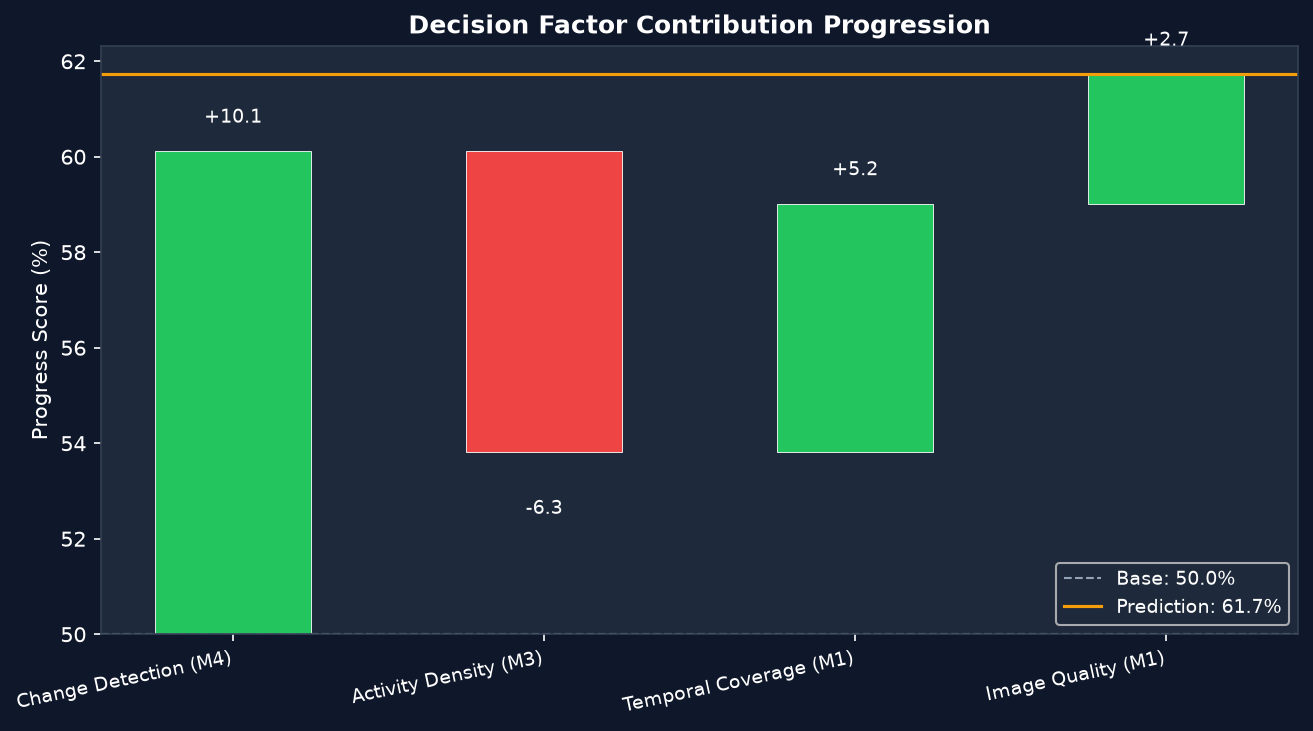
\includegraphics[width=\linewidth]{figures/shap.png}
    \caption{SHAP parametric feature attribution waterfall diagram quantifying individual factor contributions to progress variance.}
    \label{fig:shap}
\end{figure}

\subsection{Error Analysis and Failure Modes}
A detailed examination of baseline change detection errors reveals three primary operational failure modes:
\begin{enumerate}
    \item \textit{Diurnal Shadow Displacement:} Sharp shadows cast by perimeter fencing and cranes during late afternoon flights generate false-positive pixel differences that Otsu thresholding cannot fully suppress.
    \item \textit{Perspective and Parallax Distortion:} In oblique UAV captures of multi-story structures, slight variations in drone station-keeping create apparent facade displacements that mimic structural modifications.
    \item \textit{Transient Equipment Mobility:} Mobile concrete trucks and delivery vans moving across site access roads are correctly detected as changed pixels but do not correspond to permanent structural progress.
\end{enumerate}

\section{System Interface and Prototype}

The realized prototype provides an intuitive, web-based management suite accessible to field engineers via desktop or tablet browsers. The interface organizes inspection workflows into structured views: project creation, UAV image uploading with real-time quality validation feedback, interactive bi-temporal change comparison, safety compliance summaries, S-curve trajectory visualization, and automated PDF evidence report downloads. The system maintains responsive execution on lightweight field laptops without requiring external cloud connectivity.

\section{Limitations and Future Enhancements}

To maintain rigorous scientific standards, the operational limitations of the present system must be explicitly stated:
\begin{enumerate}
    \item \textit{Optical and Aerodynamic Sensitivity:} Severe atmospheric haze, rainfall, or high wind gusts can degrade UAV image sharpness below the validation threshold.
    \item \textit{Illumination Drift:} Deterministic Otsu thresholding remains vulnerable to intense solar illuminance changes and diurnal shadow movement.
    \item \textit{Planar Geometric Constraint:} 2D orthophoto differencing cannot directly measure volumetric cut-and-fill earthworks, which necessitate dense 3D photogrammetric meshing.
    \item \textit{Model Weight Availability:} Real-time asset detection requires pre-trained PyTorch weight files; in their absence, the system relies on ground-truth annotation parsing.
    \item \textit{Exterior Boundary Constraint:} Aerial UAV imaging cannot monitor interior architectural installations, MEP ductwork, or enclosed structural curing.
    \item \textit{Human Supervisory Imperative:} The system is designed strictly for decision support; final contractual and safety decisions remain the prerogative of licensed human engineers.
\end{enumerate}

Future research enhancements include:
\begin{itemize}
    \item Integrating lightweight deep Siamese change detection transformers (such as ChangeFormer) trained specifically on aerial construction sequences.
    \item Developing automated 3D Gaussian Splatting and NeRF modules to compute volumetric earthwork modifications from continuous drone video streams.
    \item Establishing bidirectional integration with 4D Building Information Models (IFC/BIM) to automatically reconcile as-built UAV observations with design geometries.
    \item Validating delay forecasting algorithms against multi-year longitudinal datasets paired with daily contractor logs.
\end{itemize}

\section{Conclusion}

This paper presented an explainable, vision-based framework for construction progress assessment and schedule delay prediction using multi-temporal UAV imagery, developed under Smart India Hackathon problem statement SIH1726. The system integrates automated image quality validation, construction activity and PPE compliance detection across ten classes, classical bi-temporal change detection, Earned Value Management schedule variance modeling, and dual-stage Explainable AI combining Grad-CAM spatial heatmaps with SHAP parametric feature attributions.

Empirical evaluation on physical benchmark datasets demonstrated a pixel accuracy of 72.85\% on SYSU-CD and 72.00\% on LEVIR-CD+, with the full evaluation executing in 5.9 seconds on standard hardware. Analysis of the Roboflow Construction Site Safety dataset (38,835 annotations across 2,799 images) quantified real-world class distributions and site safety compliance. The automated software test suite achieved a 100\% pass rate across all 159 tests. The framework produces a standardized evidence report that links physical visual evidence to contractual schedule milestones, providing an auditable, transparent tool for construction project governance.



\section*{Acknowledgment}
The authors gratefully acknowledge the Department of Computer Science and Engineering at Sri Krishna College of Engineering and Technology, Coimbatore, India, for providing computational infrastructure and technical support.

\bibliographystyle{IEEEtran}
\bibliography{references}

\end{document}
